\documentclass{article}
\usepackage{lmodern}            % Smoothly scaling font.
\usepackage[                    % Set the default font size.
fontsize=24,
]{fontsize}
\renewcommand{\familydefault}{\sfdefault}
\usepackage[
% - HP DesignJet Z5200 printer in the Chemical Engineering department
%   has a 44" roll width (1118 mm).
% - The FacultyHack @ Science Gateways 2025 conference allows 30"x45"
% - Therefore, crop the poster to 44in height i.e. 30"x44"
paperwidth=30in,
paperheight=44in,
margin=0.5cm,
head=2.47in,
foot=1.59in,
includeheadfoot,
%showframe,
]{geometry}
\usepackage{fancyhdr}
\title{GPUs for massively parallel mechanistic modeling}
\pagestyle{fancy}
\renewcommand{\headrulewidth}{0pt}
\renewcommand{\footrulewidth}{0pt}
\fancyhead[L]{%
  \begin{tikzpicture}[%
    background rectangle/.style = {
      fill = fh-blue,
    },
    show background rectangle,
    tight background,
    scale = 1]
    \node (ref) [
    minimum width = \paperwidth - 1cm,
    minimum height = 2.47in] {};
    \node at (ref.north west) [anchor = north west, name = fh] {%
      
\includegraphics[height=2.47in]{fh.png}};
    \node at (ref.south east) [%
    anchor = south east, %
    name = nsf-text,
    text = fh-gold,
    scale = 0.5,
    inner sep = 6pt,
    text width = width("under award number 2231406"),
    align = center] {%
      SGX3 is funded by the \mbox{National Science Foundation} %
      under award number 2231406};
    \path let
    \p1 = (ref.north),
    \p2 = (nsf-text.north),
    \n1 = {(\y1 - \y2) - 4pt} in
    node at (nsf-text.north) [anchor = south, name = nsf, yshift = -2pt] {%
      
\includegraphics[height=\n1]{nsf.png}};
    \node at (fh.east) [%
    anchor = west,
    text = fh-gold,
    scale = 3,
    text width = width("GPUs for massively parallel")] {%
      GPUs for massively parallel mechanistic modeling%
    };
  \end{tikzpicture}%
}
\fancyhead[C,R]{}
\fancyfoot[L]{%
  \begin{tikzpicture}[%
    background rectangle/.style = {
      fill = fh-blue,
      inner sep = 0pt,
    },
    show background rectangle,
    tight background,
    scale = 1]
    \pgfdeclarelayer{foreground}
    \pgfsetlayers{background,main,foreground}
    \begin{pgfonlayer}{foreground}
    \node (ref) [
    inner sep = 0,
    minimum width = 30in - 1cm,
    minimum height = 1.59in] {};
    \node (sgx3) at ([xshift=0.5cm]ref.west) [anchor = west] {%
      
\includegraphics[height=0.85in]{sgx3.png}};
    \node (ornl) at (sgx3.east) [anchor = west] {%
      
\includegraphics[height=1.04in]{ornl.png}};
    \node (omnibond) at (ornl.east) [anchor = west] {%
      
\includegraphics[height=0.87in]{omnibond.jpg}};
    \node (tacc) at (omnibond.east) [anchor = west] {%
      
\includegraphics[height=0.87in]{tacc.png}};
    \node (qr-code) at (ref.east) [anchor = east, outer sep = 0.25cm] {%
      
\includegraphics[height=1.32in]{qr-code.png}};
    \node at (qr-code.west) [anchor = east, text = fh-gold, scale = 1.6] {%
      \textbf{Event Site:} %
      \url{https://hackhpc.github.io/facultyhack-gateways25}
      };
    \end{pgfonlayer}
    \begin{pgfonlayer}{main}
      \node [
      inner sep = 0pt, fit = (sgx3) (ornl) (omnibond) (tacc), fill = white] {};
    \end{pgfonlayer}
  \end{tikzpicture}%
}
\fancyfoot[C]{}

\usepackage{graphicx}
\graphicspath{{img/}}

\usepackage{multicol}
\setlength{\columnseprule}{0pt}
\setlength{\columnsep}{2.5pc}

\usepackage{tikz}
\usepackage{tikz}
\tikzset{
  every node/.style = {
    inner sep = 0pt,
    outer sep = 0pt
  }
}
\usetikzlibrary{
arrows.meta,
backgrounds,
calc,
decorations.markings,
decorations.pathmorphing,
decorations.text,
fit,
mindmap,
tikzmark
}

\usepackage{soul}

\usepackage{amssymb}            % \blacksquare
\usepackage{amsmath}            % \text

\usepackage{tabularx}
\newcolumntype{C}{>{\centering\arraybackslash}X}
\newcolumntype{R}{>{\raggedleft\arraybackslash}X}
% Vertically center within row https://tex.stackexchange.com/a/343329
\renewcommand\tabularxcolumn[1]{m{#1}}
\usepackage{booktabs}
\usepackage{multirow}

\usepackage[
abbreviate=true,
bibencoding=utf8,
minnames=2,
maxbibnames=99,
sorting=none,
style=vancouver,
citestyle=numeric-comp,
url=false,
]{biblatex}
% The vancouver citation style is based on NLM per
% https://tex.stackexchange.com/a/371433
\addbibresource{references.bib}
\renewcommand*{\bibfont}{\footnotesize\selectfont}

\usepackage[
table
]{xcolor}
\definecolor{fh-blue-lighter}{HTML}{EBEFF7}
\definecolor{fh-blue-darker}{HTML}{D4DEED}
\definecolor{fh-blue}{RGB}{0,89,157}
\definecolor{fh-gold}{HTML}{F7E8C9}

\usepackage{tcolorbox}
\tcbuselibrary{poster}
\newcommand{\sectionbox}[1]{%
  \begin{tcolorbox}[sharp corners,boxrule=0pt,top=15pt,colback=fh-blue,coltext=fh-gold]%
    \section*{#1\vphantom{Yy}}%
  \end{tcolorbox}%
}

% Reduce excessive hyphenation https://stackoverflow.com/a/65156105
\tolerance=9999
\emergencystretch=10pt
\hyphenpenalty=10000
\exhyphenpenalty=100

\begin{document}

\noindent
\begin{tcbposter}[
  poster = {
    rows = 1,
    columns = 2,
    height = \paperheight - 2cm - 2.47in - 1.59in,
    width = \paperwidth - 1cm,
    colspacing = 0.1in,
    rowspacing = 0.1in,
    %showframe,
  },
  boxes = {
    fonttitle = \Large\bfseries,
    coltitle = fh-gold,
    colbacktitle = fh-blue,
    colback = white,
    colframe = white,
    sharp corners,
    boxrule = 0pt,
  },
  ]

  \posterbox[
  adjusted title = Introduction,
  ]{
    name = intro,
    column = 1,
  }{%
  \noindent
  Graphical Processing Units (GPUs) %
  are integrated into the core architecture %
  of the world's fastest supercomputers %
  that solve the most computationally difficult, %
  mechanistic scientific problems.
  %
  An 8~year, \$1.8~billion effort %
  called the Exascale Computing Project (ECP) %
  involving 2,800 scientists and engineers %
  recently finished modernizing %
  the underlying scientific numerical software %
  to efficiently use this new generation of machines.
  \smallskip

  \noindent
  Computing facilities grant access at no cost %
  to these GPU-accelerated%
  \supercite{%
    carter_2014,%
    beckingsale_2019,%
    reinders_2023%
  } machines %
  only to research software engineers and scientists who demonstrate that %
  their computations scale %
  to efficiently use multiple GPUs across many computer servers / nodes.
  %
  Therefore, %
  it is imperative to teach %
  the data parallel software development skills, %
  appropriate domain science methods, and %
  sustainable software practices %
  to enable large scale, GPU-centric computational research.
  \smallskip

  \noindent
  Discussion and feedback on this poster from the community %
  can help make this course a success and %
  support similar hands-on learning and teaching endeavors.
  \smallskip

  \noindent
  \begin{minipage}[c]{.36\linewidth}
    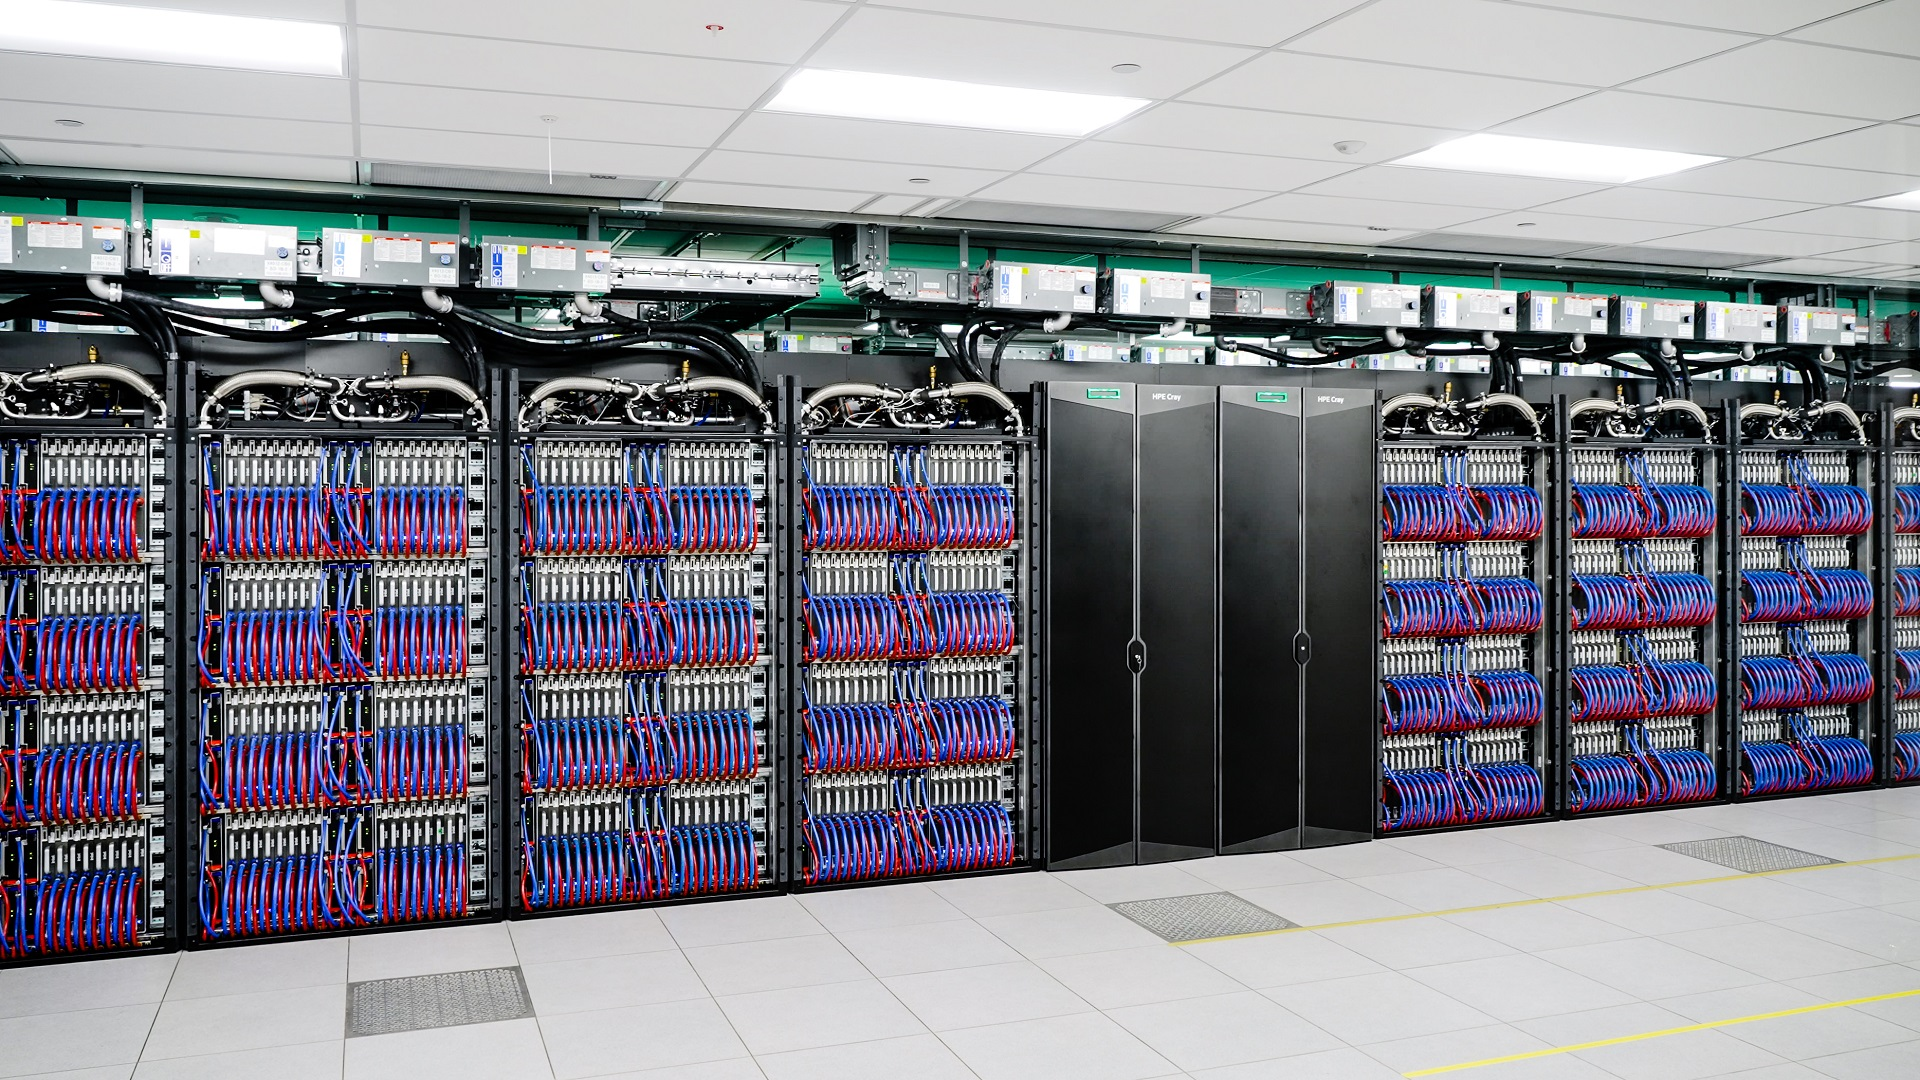
\includegraphics[width=\linewidth]{1920x1080-Aurora hero image.jpg}
  \end{minipage}
  \begin{minipage}[c]{.62\linewidth}
    \textbf{Modern supercomputers use GPU architectures.}
    %
    Left photo is the Aurora supercomputer at Argonne National Laboratory %
    that is ranked 3\textsuperscript{rd} in the Top 500 List of June 2025 %
    and one of three US exascale supercomputers.
    %
    Germany recently launched their first exascale supercomputer, JUPITER, %
    and China may have as many as 10 exascale supercomputers %
    by the end of this year\supercite{dongarra_2023} %
    but stopped submitting data to the Top 500 List %
    after US GPU embargoes.
  \end{minipage}

  \vspace{-.5\baselineskip}
  \subsection*{\textcolor{fh-blue}{Target Course Description}}
  \vspace{-.5\baselineskip}
  {
    \rowcolors{1}{fh-blue-lighter}{fh-blue-darker}
    \begin{tabularx}{\linewidth}{>{\bfseries}r X}
      \toprule
      Course Name:
      & GPUs for massively parallel mechanistic modeling\\
      Course Number:
      & TBA\\
      Department:
      & Chemical Engineering\\
      Anticipated Enrollment:
      & 12\\
      Prerequisites:
      & fluent with at least one %
      procedural programming language\\
      Key Content:
      & performance optimization, %
      software development, %
      domain science methods, %
      capstone project\\
      Description:
      & This course trains graduate researchers %
      with ECP-level skills in high performance computing (HPC), %
      using research software engineer (RSE) rigor, %
      and HPC-relevant domain scientific methods.\\
      Project Repo:
      & \small \url{https://github.com/omsai/facultyhack-gateways25-nanda}\\
      \bottomrule
    \end{tabularx}
  }

  \vspace{-\baselineskip}
  \subsection*{\textcolor{fh-blue}{Goals}}
  \vspace{-.5\baselineskip}
  \begin{itemize}
  \setlength{\itemsep}{-.5em}
  \item Setup student \ul{JetStream2 VM} for homework and capstone projects.
  \item Add students to my \ul{ACCESS group} for cluster runs and %
    help them get their own ACCESS allocation.
  \item Teach all C++ classroom exercises inside a \ul{web IDE}. 
  \item Train students to \ul{package their project}.
  \end{itemize}
  }

  \posterbox[
  adjusted title = Initial Course Syllabus,
  ]{
    name = syl-init,
    column = 1,
    below = intro,
  }{%
  \noindent
  This course was inspired by the %
  2024 Argonne Training Program on Extreme-Scale Computing (ATPESC'24) %
  and the 2025 LLNL %
  High Performance Computing Innovation Center (HPC-IC'25) %
  tutorial series.
  \medskip

    \noindent
    \begin{tabularx}{\linewidth}{%
      >{\hsize=.15\hsize\linewidth=\hsize}X %
      >{\hsize=.34\hsize\linewidth=\hsize}R %
      >{\hsize=.16\hsize\linewidth=\hsize}C %
      >{\hsize=.16\hsize\linewidth=\hsize}C %
      >{\hsize=.16\hsize\linewidth=\hsize}C}
      \toprule
      \textbf{Category}
      & \textbf{Topic}
      & \textbf{This Course} & \textbf{ATPESC'24} & \textbf{HPC-IC'25}\\
      \midrule
      \multirow{4}{\hsize}{Performance optimization
      \textcolor{orange!90!black}{$\blacksquare$}}
      & Within node
      & \checkmark & \checkmark & $\times$\\
      & Multi-node
      & \checkmark & \checkmark & \checkmark\\
      & GPU performance portability
      & \checkmark & \checkmark & \checkmark\\
      & Performance tuning
      & \checkmark & \checkmark & \checkmark\\
      \midrule
      \multirow{9}{\hsize}{Software development
      \textcolor{blue!80!black}{$\blacksquare$}}
      & Unit testing
      & \checkmark & \checkmark & $\times$\\
      & Performance testing
      & \checkmark & \checkmark & \checkmark\\
      & CI, checkpointing, benchmarking
      & \checkmark & $\times$ & \checkmark\\
      & Parallel debugging
      & \checkmark & \checkmark & $\times$\\
      & Code peer review, documentation
      & \checkmark & $\times$ & $\times$\\
      & Packaging
      & \checkmark & \checkmark & \checkmark\\
      \midrule
      \multirow{-0.5}{\hsize}{Domain science methods
      \textcolor{green!50!black}{$\blacksquare$}}
      & Mechanistic multiscale modeling
      & \checkmark & $\times$ & $\times$\\
      & Scientific parameter fitting
      & \checkmark & $\times$ & $\times$\\
      & Coupling AI, cloud, data science
      & \checkmark & $\times$ & \checkmark\\
      \midrule
      \multirow{2}{\hsize}{Sysadmin
      \textcolor{black!60}{$\blacksquare$}}
      & Cluster launch
      & \checkmark & $\times$ & \checkmark\\
      & Cluster profiling
      & \checkmark & \checkmark & \checkmark\\
    \end{tabularx}
  }

  \posterbox[
  adjusted title = Mentors Suggestions,
  ]{
    name = sugg,
    column = 1,
    below = syl-init,
  }{%
  \begin{multicols}{2}
    \begin{enumerate}
    \setlength{\itemsep}{0em}
    \item \ul{Added network communication exercises} %
      using the LAMMPS exercise developed at Temple University.
    \item \ul{Added profiling exercises} %
      from Cornell University %
      and the University of Michigan.
    \item \ul{Chose a checkpointing library} %
      written in C++ %
      both to teach in the course %
      and to recommend for student capstone projects.
    \item Trainees will \ul{write C++ code using VS Code} %
      with SSH tunnels to JetStream2 virtual machines %
      with a fallback of OpenVSCode Server web interface %
      for classroom instruction.
    \item \ul{Added AI policy} %
      requiring a bibliography %
      citing AI service names with versions, prompts, and output.
    \item Moved non-capstone homework assignments to %
      \ul{classroom hands-on to avoid over-reliance on AI support} %
      while trainees are still developing expertise.
    \item \ul{Increased accessibility} %
      for non-C++ programmers %
      by recommending self-guided, open access textbooks %
      from \emph{The Art of HPC: Volume 3}.
    \item \ul{Added objective of numerical correctness} %
      but limited goal to unit tests, performance test, and CI %
      instead of considering formal methods.
    \item The target audience is now \ul{graduate students} %
      with existing projects or pilot projects.
    \item \ul{Consolidated course topics} %
      to focus on domain science methods %
      in keeping with the course title.
    \end{enumerate}
  \end{multicols}
  }

  \posterbox[
  adjusted title = Science Gateways Resources Used,
  ]{
    name = res,
    column = 1,
    below = sugg,
  }{%
  \begin{multicols}{2}
    \begin{tikzpicture}
      \node (text) %
      [text width = .6\linewidth] {%
        \textbf{Non-virtual multi-GPU A100 nodes (g3.2xl)}};
      \node (logo) at (text.south east) %
      [anchor = south west, minimum width = .4\linewidth] {%
        
\includegraphics[width=.4\linewidth]{jetstream2-head-logo.pdf}};
    \end{tikzpicture}
    \vspace{-1.5\baselineskip}
    \begin{itemize}
    \setlength{\itemsep}{-.5em}
    \item Shared between small groups of 4 students.
    \item For early project development and exercises.
    \item A100 supports 64-bit floating point operations %
      for capstone projects that may require it.
    \item Efficient multi-GPU use is a course objective.
    \item g3.2xl is the multi-GPU A100 with the most availability.
    \end{itemize}

    \begin{tikzpicture}
      \node (text) %
      [text width = .6\linewidth] {%
        \textbf{Bridges-2 GPU HPC allocation}};
      \node (logo) at (text.south east) %
      [anchor = south west, minimum width = .4\linewidth] {%
        
\includegraphics[width=.4\linewidth]{access-logo.pdf}};
    \end{tikzpicture}
    \vspace{-1.5\baselineskip}
    \begin{itemize}
    \setlength{\itemsep}{-.5em}
    \item For cluster exercises and scaling.
    \item Interactive nodes with backfill scheduling and short walltime %
    for the classroom use.
    \item Trainees are encouraged %
    to apply for their own ACCESS CI allocations %
    to continue their work %
    after leaving the instructor's ACCESS CI group.
    \end{itemize}

    \begin{tikzpicture}
      \node (text) %
      [text width = .6\linewidth] {%
        \textbf{HPC introduction and reproducible workflows}};
      \node (logo) at (text.south east) %
      [anchor = south west, minimum width = .4\linewidth] {%
        
\includegraphics[width=.4\linewidth]{hpc-carpentry.pdf}};
    \end{tikzpicture}
    \vspace{-1.5\baselineskip}
    \begin{itemize}
    \setlength{\itemsep}{-.5em}
    \item Self-paced introduction to key concepts of the  HPC environment.
    \item Supplementary reading for %
      capstone project reproducible workflows %
      for coupling AI, cloud, and data science tools.
    \end{itemize}

    \begin{tikzpicture}
      \node (text) %
      [text width = .6\linewidth] {%
        \textbf{%
          Trainee GitHub repositories for assignments and capstone projects}};
      \node (logo) at (text.south east) %
      [anchor = south west, minimum width = .4\linewidth] {%
        
\includegraphics[width=.2\linewidth]{github-mark.pdf}
        
\includegraphics[width=.2\linewidth]{actions-icon-actions.pdf}
      };
    \end{tikzpicture}
    \vspace{-1.5\baselineskip}
    \begin{itemize}
    \setlength{\itemsep}{-.5em}
    \item Projects in private git repositories shared with the instructor.
    \item Assignments partially checked using GitHub actions.
    \item Progress on capstone projects will be monitored from git repositories.
    \end{itemize}
  \end{multicols}
  }

  \posterbox[
  adjusted title = Modified Course Syllabus,
  ]{
    name = syl-modified,
    column = 2,
  }{%
    The topics covered in this course %
    are organized into the categories of the %
    \textcolor{red!80!black}{$\blacksquare$}~capstone project,
    \textcolor{orange!90!black}{$\blacksquare$}~performance optimization, %
    \textcolor{blue!80!black}{$\blacksquare$}~software development, %
    \textcolor{green!50!black}{$\blacksquare$}~domain science methods, and %
    \textcolor{black!60}{$\blacksquare$}~cluster administration.
    % 
    Each item more-or-less corresponds to %
    a single week of semester classroom sessions.
    %
    To accommodate delays from needing to spend extra time clarifying
    critical topics taught earlier in the class, two class weeks can be
    dropped and have been marked with ``(Time permitting)''.
    \begin{multicols}{2}
      \begin{itemize}
      \item[\textcolor{red!80!black}{$\blacksquare$}] \textbf{Write
          abstract:} begin a capstone project after completing the
        performance optimization topics\\
        \textbf{Assignment 0:} Write a half page proposal for a new or
        existing compute-intensive mechanistic model to be accelerated
        using GPU resources.%
      \item[\textcolor{orange!90!black}{$\blacksquare$}]
        \textbf{Within-node optimization:} strategies for within-node
        vectorization, caching, memory bandwidth, and I/O\\
        \textbf{Assignment 1:} Exercises vectorizing Python code,
        inspecting C assembler CPU vectorized instructions, creating
        roofline plots to inspect CPU-memory, hwloc to inspect memory
        CPU hierarchy.%
      \item[\textcolor{orange!90!black}{$\blacksquare$}]
        \textbf{Multi-node scaling:} strategies for task distribution
        and multi-node cluster scaling\\
        \textbf{Assignment 2:} Exercises with C, TaskWorks, Spack,
        MPI, and SLURM.%
      \item[\textcolor{orange!90!black}{$\blacksquare$}] \textbf{GPU
          acceleration:} introduction to data parallel programming for
        GPUs\\
        \textbf{Assignment 3:} Exercises with C++ Kokkos to fill in
        the blanks of partially completed programs.\\
        \textbf{Assignment 3-capstone:} Outline an informal list of
        goals and objectives to create a minimum viable product of
        your capstone code through the remainder of the semester.%
      \item[\textcolor{orange!90!black}{$\blacksquare$}] \textbf{
          Distributed performance tuning:} Introduction to distributed
        performance tuning\\
        \textbf{Assignment 4:} Exercises with Darashan, Drishti, and
        HPCtoolkit\\
        \textbf{Assignment 4-capstone:} Literature review of software
        similar to yours and how you intend to make yours different.%
      \item[\textcolor{blue!80!black}{$\blacksquare$}] \textbf{
          Testing, CI, and benchmarking}: automated unit testing,
        performance regression testing, test coverage, and continuous
        integration\\
        \textbf{Hands-On 5}: Exercises with pytest, Benchpark, and
        GitLab CI.\@\\
        \textbf{Assignment 5-capstone:} Start adding tests, coverage,
        and CI to your capstone project.%
      \item[\textcolor{blue!80!black}{$\blacksquare$}] \textbf{ Peer
          review, usability, packaging:} practicing stress-free code
        peer review, documentation, and packaging\\
        \textbf{Hands-On 7:} Exercise with professor and pairing.\\
        \textbf{Assignment 7-capstone:} Document, package with Spack
        or Apptainer.%
      \item[\textcolor{blue!80!black}{$\blacksquare$}] \textbf{
          Parallel debugging and checkpointing:} introduction to
        parallel
        debugging, code correctness, and application checkpoints\\
        \textbf{Hands-On 6:} MPIGDB debugging session, resuming from
        checkpoint
        to understand error, correctness with sanitizers.\@\\
        \textbf{Assignment 6-capstone:} Start adding checkpointing to
        your capstone project.%
      \item[\textcolor{green!50!black}{$\blacksquare$}] \textbf{
          Mechanistic, multiscale modeling:} simulations using an
        agent-based, mechanistic, multiscale model\\
        \textbf{Hands-On 8:} Analyze how model layers and linking are
        implemented\supercite{cilfone_2015}.%
      \item[\textcolor{green!50!black}{$\blacksquare$}] \textbf{
          Parallel parameter fitting:} parallel parameter fitting
        using gradient-free, pseudo-likelihood based sampling\\
        \textbf{Hands-On 9:} Calibrating our model from last time with
        pyabc using adaptive sampling; discuss
        checkpointing, debugging.\\
        \textbf{Assignment 9-capstone:} Start coupling with scientific
        parameter sampling.%
      \item[\textcolor{green!50!black}{$\blacksquare$}] (Time
        permitting) \textbf{Coupling AI, cloud, data science:}
        Coupling HPC
        paradigms with data science, AI, and cloud environments\\
        Assignment 10: Summarize book\supercite{zbakh_2024} chapters 4
        and 8 in 1 page.\\
        \textbf{Assignment 10-capstone:} Assess possible extensions to
        your capstone project using components of AI, big data, or
        cloud applications and specialized hardware needs by
        connecting the concepts from each of the two articles, your
        domain science, and to what extent we discussed these concepts
        so far in the class.%
      \item[\textcolor{black!60}{$\blacksquare$}] (Time permitting)
        \textbf{Cluster sysadmin and profiling:} cluster launch,
        system
        administration, and profiling\\
        \textbf{Hands-On 11:} Setup VMs with network, shared disk, and
        SLURM to launch and profile an ad-hoc, suboptimal cluster.%
      \item[\textcolor{red!80!black}{$\blacksquare$}] \textbf{Final
          presentations and code:} final presentations of capstone
        projects\\
        \textbf{Hands-On 12-capstone:} Walk though your project with
        ACCESS-relevant details and future directions.\\
        \textbf{Assignment 12-capstone:} Submit code for grading.%
      \item[\textcolor{red!80!black}{$\blacksquare$}] \textbf{NSF
          ACCESS proposal:} NSF ACCESS allocation request\\
        \textbf{Assignment 13-capstone:} Write a 3-page ACCESS CI
        Accelerate proposal with scaling studies and justification for
        compute resources requested; trim actual Discover proposal to
        1-page.%
      \end{itemize}
    \end{multicols}
  }

  \posterbox[
  adjusted title = Expansions,
  ]{
    name = exp,
    column = 2,
    below = syl-modified,
  }{%
  \begin{multicols}{2}
    \begin{enumerate}
    \setlength{\itemsep}{0em}
    \item Accommodate \ul{undergraduate students} %
      with more structure, %
      shorter exercises, %
      and allow them to choose from a set of smaller capstone projects.
    \item For the last ``fun'' topic before final presentations %
      \ul{launch the cluster using Raspberry Pis}, %
      networking hardware, and network storage %
      for a more memorable hands-on lesson.
    \item Develop an \ul{time-saving exercise for model comparison} %
      to demonstrate the usefulness %
      of detailed benchmarking and analysis tools %
      \ul{to rapidly iterate model development}.
    \item Create \ul{interactive trivial exercises in a web page} %
      to encourage trainee progress with %
      a live updating grading rubric %
      and suggestions to correct common errors.
    \item \ul{Compartmentalize topics %
      into the 2-day workshop format} %
      to be taught at the Pittsburgh Supercomputing Center (PSC).
    \item Create \ul{HPC Carpentry lessons in C++ for data scientists}
      to cover C++ concepts required to use GPU performance
      portability libraries by comparing to concepts in Python and R
      where possible, namely: variables, functions, data structures,
      loops, classes (constructors, member variables, member
      functions, member operators), debugging.
    \end{enumerate}
  \end{multicols}
  }

  \posterbox[
  adjusted title = References,
  ]{
    name = references,
    column = 2,
    below = exp,
  }{%
  {
    % Recalculate \columnsep instead of using the large \columnsep
    % from the main document.
    \setlength{\columnsep}{1.5pc}
    \begin{multicols}{2}
      \printbibliography[heading=none]{}
    \end{multicols}
  }
  }

  \posterbox[
  adjusted title = Authors,
  ]{
    name = authors,
    column = 2,
    below = references,
  }{%
  \begin{tikzpicture}
    \node (pn) {%
    \includegraphics[%
    keepaspectratio,
    width=10em,
    height=5em,
    clip,
    trim={55 85 50 35}]{%
        pariksheet.png}};

    \node (pn-text) at (pn.north east) [anchor = north west, xshift = 0.5em, align = left] {%
      \textcolor{fh-blue}{\tikzmark{pn}Nanda, Pariksheet}\\
      Role: Faculty Participant\\
      University of Pittsburgh\\
      pan79@pitt.edu
    };

    \node (em) at ($ (pn.north west) + (.5\linewidth,0) $) [%
    anchor = north west,
    xshift = 1em] {%
      \includegraphics[%
      keepaspectratio,
      width=10em,
      height=5em,
      clip,
      trim={20 80 60 5}]{%
        elijah.jpg}};

    \node at (em.north east) [anchor = north west, xshift = 0.5em, align = left] {%
      \textcolor{fh-blue}{\tikzmark{pn}MacCarthy, Elijah}\\
      Role: Community Mentor\\
      Oak Ridge National Laboratory\\
      maccarthyea@ornl.gov
    };
  \end{tikzpicture}
  }

\end{tcbposter}

\end{document}
